\documentclass{standalone}

\usepackage{tikz}
\usetikzlibrary{calc}

\begin{document}
    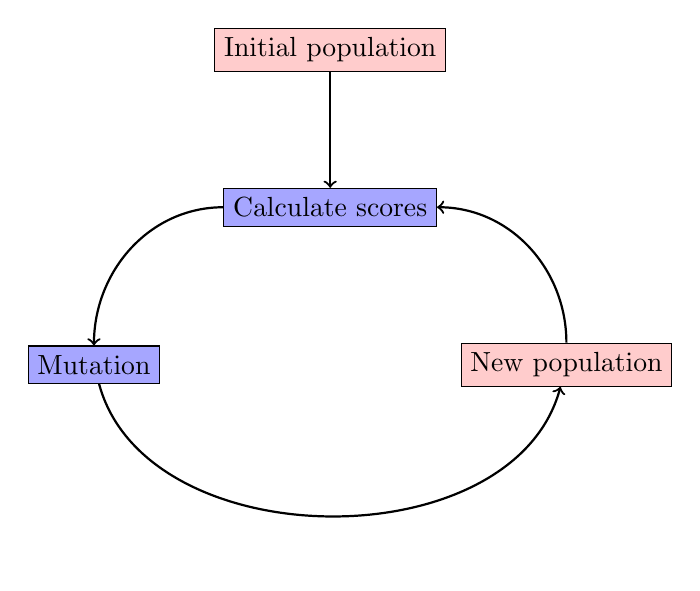
\begin{tikzpicture}
        \node (initial) at (0, 0) [fill=red!20, draw] {Initial population};

        \node (fitness) at ($(initial) + (0, -2)$) [fill=blue!35, draw] {Calculate scores};

        \node (mutation) at ($(fitness) + (-3, -2)$) [fill=blue!35, draw] {Mutation};
        \node (new) at ($(mutation) + (6, 0)$) [fill=red!20, draw] {New
            population};

        \draw [->, thick] (initial) -- (fitness);
        \draw [->, thick] (fitness) to [out=180, in=90] (mutation);
        \draw [->, thick] (mutation) to [out=-75, in=-105] (new);
        \draw [->, thick] (new) to [out=90, in=0] (fitness);
    \end{tikzpicture}
\end{document}
